\subsection(definisi)
operasi pembagian pada dasarnya adalah 
suatu proses pencarian tentang bilangan yang belumdiketahui. Karena bentuk pembagian dapat dipandang atau dilihat sebagai suatu bentuk operasi perkalian dengan salah satu faktornya yang belum diketahui

\subsection(SEJARAH)
Penemuan ini,  telah dirancang untuk memecahkan masalah dan objeknya adalah untuk menyediakan pembagi yang dapat melakukan pembagian dengan pembagi 
dan semua pembagi menjadi bilangan heksadesimal. Pembagi dari penemuan ini dibuat untuk menyelaraskan digit dari pembagi normalisasi normalisasi di muka 
dengan secara selektif menggunakan fungsi pergeseran dan fungsi pergeseran yang tepat yang dibangun pada pemilih, 
dan kemudian menentukan hasil pembagian heksadesimal dengan mengulangi proses dengan menentukan nomor kali.

Penemuan pertama pembagi yang terkait dengan penemuan ini dilengkapi dengan rangkaian normalisasi pertama untuk memasukkan data dari data floating point pembagi yang basisnya 16 dan menormalisasinya berdasarkan basis di atas, 
rangkaian normalisasi kedua untuk memasukkan data dari Pembagi adalah data floating point yang basisnya adalah 16 dan menormalisasinya berdasarkan basis di atas, rangkaian pembagi, 
dan pemilih untuk memasukkan data mantissa dari pembagi dari rangkaian normalisasi pertama, 
sisa data dari rangkaian pemisah dan sinyal siklus divisi yang menunjukkan siklus divisi, dan ketika sinyal siklus divisi menunjukkan siklus pertama,
melalui-keluaran data mantissa dari pembagian secara utuh, ketika sinyal siklus divisi menunjukkan siklus kedua dan data mantissa di bagi sama dengan atau lebih besar dari pada pembagi, 
menggeser data mantissa dari pembagi ke kanan dan mengeluarkannya, 
ketika sinyal siklus divisi menunjukkan siklus kedua dan mantiss data di bagi lebih kecil dari pada pembagi, 
menggeser data mantissa dari dividen ke kiri dan mengeluarkannya,
dan ketika sinyal siklus divisi menunjukkan siklus ketiga dan setelah ketiga, melalui pengeluaran data sisa utuh, 
dimana pembagi rangkaian menghitung data hasil bagi dan data sisa dari data yang dikeluarkan oleh pemilih dan data mantissa dari pembagi yang dikeluarkan oleh rangkaian normalisasi kedua.

Menurut penemuan kedua pembagi yang terkait dengan penemuan ini, shifter kiri di sirkuit pemisah biasanya digunakan di tempat shifter kiri yang diperlukan pada pemilih pada penemuan pertama oleh fakta bahwa selektor pembagi yang terkait dengan penemuan ini dibangun sedemikian rupa sehingga, 
ketika sinyal siklus divisi menunjukkan siklus pertama, ia mengeluarkan data mantissa dari dividen, ketika sinyal siklus divisi menunjukkan siklus kedua dan data mantissa dividen sama atau lebih besar dari pada pembagi , 
itu menggeser data mantissa dari dividen menjadi ketakutan dan mengeluarkannya, dan ketika sinyal siklus divisi menunjukkan siklus kedua dan data mantissa dividen lebih kecil dari pada pembagi atau ketika sinyal siklus divisi menunjukkan yang ketiga dan setelahnya siklus ketiga, itu data sisa sisa.

\subsection{Bilangan Biner}
Sejak pertama kali komputer elektronik digunakan, komputer beroperasi dengan menggunakan bilangan biner, yaitu bilangan dengan basis 2 pada sistem bilangan. Semua kode program dan data pada komputer disimpan serta dimanipulasi dalam format biner yang merupakan kode-kode mesin komputer. Sehingga semua per-hitungannya diolah menggunakan aritmatik biner, yaitu bilangan yang hanya memiliki nilai dua kemungkinan yaitu 0 dan 1 dan sering disebut sebagai bit (binary digit atau dalam arsitektur elektronik biasa disebut sebagai digital logic. Representasi bilangan biner bas dilihat disamping ini. Posisi sebuah angka akan menentukan berapa bobot nilainya. Posisi paling depan (kiri) sebuah bilangan memiliki nilai yang paling besar sehingga disebut sebarai MSB (Most Significant Bit), dan posisi paling belakang (kanan) sebuah bilangan memiliki nilai yang paling kecil sehinggal disebut sebagai LSB (Leased Significant Bit).

Contoh: reprentasi bilangan dengan basis biner:
\begin{equation}
101102 = 1*2^4 + 0*2^3+1*2^1+0*2^0=2210
\end{equation}

\subsection{Bilangan Heksadesimal}
Bilangan heksadesimal atau biasa disebut heksa saja, berbasis 16 memiliki nilai yang disimbolkan dengan 0, 1, 2, 3, 4, 5, 6, 7, 8, 9, a, b, c, d, e, f. Adanya bilanagn ini dikarenakan operasi bilangan biner untuk data yang lebih besar akan menjadi susah, hingga bilangan ini sering digunakan untuk menggambarkan memori computer atau intruksi. Setiap digit bilangan heksa mewakili 4 bit bilangan biner, dan 2 digit bilangan heksadesimal mewakili satu byte.
Sebagai contoh bilangan hexa 41 (2 nible), pada format ASCII mewakili karakter “A”, bilangan hexa 42 mewakili karakter “B”, dan segabainya.
\subsubsection{konversi}
Untuk mengkonversinya ke dalam bilangan desimal, dapat menggunakan formula berikut:
Dari bilangan heksadesimal H yang merupakan untai digit hn hn-1… h2 h1 h0, jika dikonversikan menjadi bilangan desimal D, maka seperti gambar \ref{rumus}
\begin{figure}[ht]
	\centerline{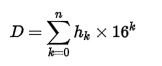
\includegraphics[width=1\textwidth]{figures/rumus.jpg}}
	\caption{rumus}
	\label{rumus}
	\end{figure}
Sebagai contoh, bilangan heksa 10E yang akan dikonversi ke dalam bilangan desimal:
\begin{itemize}
\item Digit-digit 10E dapat dipisahkan dan mengganti bilangan A sampai F (jika terdapat) menjadi bilangan desimal padanannya. Pada contoh ini, 10E diubah menjadi barisan: 1,0,14 (E = 14 dalam basis 16)
\item Mengalikan dari tiap digit terhadap nilai tempatnya.
\end{itemize}
\begin{equation}
1 x 16^2 + 0 x 16^1 + 14 x 16^0
= 256 + 0 + 14
= 270
\end{equation}
Dengan demikian, bilangan 10E heksadesimal sama dengan bilangan desimal 270.


\subsection(contoh2 operasi bilangan)
Sebagai contoh apabila dalam perkalian 3 x 4 = k tentu k = 12 maka, dalam pembagian hal tersebut dapat dinyatakan,dengan bentuk 12 : 3 = n atau 12 : 4 = n
Dengan demikian 12 : 3 = n apabila dinyatakan dalam bentuk perkalian akan menjadi 12 = n x 3, sedangkan 12 : 4 = n menjadi bentuk perkalian menjadi 12 = n x 4. Untuk mencari nilai n dari bentuk 12 = n x 3, sama artinya dengan mencari jawab pertanyaan : bilangan manakah yang jika dikalikan dengan 3 akan menghasilkan 12 atau berapakah 12 : 3  Dua pertanyaan ini mungkin akan menghasilkan bilangan yang sama. Jadi apabila dalam pertanyaan yang pertama mendapatkan nilai 4, maka berarti pula nilai dari 12 : 3 = 4.
Pembagian bilangan bulat juga dapat dikelompokan menjadi empat, yaitu:
a. Pembagian antara bilangan bulat positif dengan bilangan bulat positif 
b. Pembagian antara bilangan bulat positif dengan bilangan bulat negatif 
c. Pembagian antara bilangan bulat negatif dengan bilangan bulat positif 
d. Pembagian antara bilangan bulat negatif dengan bilangan bulat negatif Sama seperti pada operasi perkalian, pada operasi pembagian di kajian teoritis ini penulis hanya memaparkan operasi pembagian bilangan bulat positif dengan bilangan bulat positif
Untuk mendapatkan hasil pembagian bilangan bulat positif dengan bilangan bulat positif, yaitu dengan cara menggunakan pengurangan berulang sampai sisanya adalah nol. Hasil pembagian ditunjukkan dengan berapa banyak dikurangi dengan bilangan yang sama. Selanjutnya perhatikan contoh berikut ini: a. 10: 2= 10 - 2 - 2 - 2 - 2 - 2= 0 10 dikurangi 2 sebanyak 5 kali sampai sisanya 0. Artinya hasil dari 10 : 2 adalah 5. b. 24 : 4 = 24 - 4 - 4 - 4 - 4 - 4 - 4 = 0 24 dikurangi 4 sebanyak 6 kali sampai sisanya nol.
 Artinya hasilnya adalah 6. Operasi pembagian bilangan bulat positif dengan bilangan bulat positif dapat juga diperagakan dengan menggunakan garis bilangan. Untuk peragaan pada garis bilangan, kita ambil contoh pembagian berikut : 10 : 2. Untuk menentukan hasil pembagian tersebut dengan menggunakan garis bilangan adalah sebagai berikut. a. Siswa panah berkedudukan awal pada skala nol. b. Bilangan pembaginya adalah bilangan positif, maka ujung siswa panah akan menghadap ke arah bilangan positif. c. Siswa panah bergerak meloncat maju dengan setiap loncatan 2 skala, sebanyak 5 kali dan berhenti pada skala 10. d. Hasil pembagian 10 : 2 ditunjukkan dengan loncatan siswa panah sebanyak 5 loncatan maju yang berhenti pada skala 10. e. Jadi hasil dari 10 : 2 adalah 5.

